%%%%%%%%%%%%%%%%%%%%%%%%%%%%%%%%%%%%%%%%%%
% L1 - Villebon Charpak
%%%%%%%%%%%%%%%%%%%%%%%%%%%%%%%%%%%%%%%%%%
%	Régimes transitoires
%%%%%%%%%%%%%%%%%%%%%%%%%%%%%%%%%%%%%%%%%%
%
% Created by:
%	Julien VILLEMEJANE - 01/jun/2024
% Modified by:
%	
%
%%%%%%%%%%%%%%%%%%%%%%%%%%%%%%%%%%%%%%%%%%
% Professional Newsletter Template
% LaTeX Template
% Version 1.0 (09/03/14)
%
% Created by:
% Bob Kerstetter (https://www.tug.org/texshowcase/) and extensively modified by:
% Vel (vel@latextemplates.com)
% 
% This template has been downloaded from:
% http://www.LaTeXTemplates.com
%
% License:
% CC BY-NC-SA 3.0 (http://creativecommons.org/licenses/by-nc-sa/3.0/)
%
%%%%%%%%%%%%%%%%%%%%%%%%%%%%%%%%%%%%%%%%%

\documentclass[11pt]{article} % The default font size is 10pt; 11pt and 12pt are alternatives

%%%%%%%%%%%%%%%%%%%%%%%%%%%%%%%%%%%%%%%%%
% Professional Newsletter Template
% Structural Definitions File
% Version 1.0 (09/03/14)
%
% Created by:
% Vel (vel@latextemplates.com)
% 
% This file has been downloaded from:
% http://www.LaTeXTemplates.com
%
% License:
% CC BY-NC-SA 3.0 (http://creativecommons.org/licenses/by-nc-sa/3.0/)
%
%%%%%%%%%%%%%%%%%%%%%%%%%%%%%%%%%%%%%%%%%

%----------------------------------------------------------------------------------------
%	REQUIRED PACKAGES
%----------------------------------------------------------------------------------------

\usepackage{graphicx} % Required for including images
\usepackage{microtype} % Improved typography
\usepackage{multicol} % Used for the two-column layout of the document
\usepackage{booktabs} % Required for nice horizontal rules in tables
\usepackage{wrapfig} % Required for in-line images
\usepackage{float} % Required for forcing figures not to float with the [H] parameter

%------------------------------------------------
% Fonts

\usepackage{charter} % Use the Charter font as the main document font
\usepackage{courier} % Use the Courier font for \texttt (monospaced) only
\usepackage[T1]{fontenc} % Use T1 font encoding
\usepackage{lmodern}

%------------------------------------------------
% List Separation

\usepackage{enumitem} % Required to customize the list environments
\setlist{noitemsep,nolistsep} % Remove spacing before, after and within lists for a compact look

%------------------------------------------------
% Figure and Table Caption Styles

\usepackage{caption} % Required for changing caption styles
\captionsetup[table]{labelfont={bf,sf},labelsep=period,justification=justified} % Specify the table caption style
\captionsetup[figure]{labelfont={sf,bf},labelsep=period,justification=justified, font=small} % Specify the figure caption style
\setlength{\abovecaptionskip}{10pt} % Whitespace above captions

%------------------------------------------------
% Spacing Between Paragraphs

\makeatletter
\usepackage{parskip}
\setlength{\parskip}{6pt}
\newcommand{\@minipagerestore}{\setlength{\parskip}{6pt}}
\makeatother

%----------------------------------------------------------------------------------------
%	PAGE MARGINS AND SPACINGS
%----------------------------------------------------------------------------------------

\textwidth = 7 in % Text width
\textheight = 10 in % Text height
\oddsidemargin = -18pt % Left side margin on odd pages
\evensidemargin = -18pt % Left side margin on even pages
\topmargin = -36pt % Top margin
\headheight = 0pt % Remove the header by setting its space to 0
\headsep = 0pt % Remove the space between the header and top of the page
\parskip = 4pt % Space between paragraph
\parindent = 0.0in % Paragraph indentation
\pagestyle{empty} % Disable page numbering

%----------------------------------------------------------------------------------------
%	COLORS
%----------------------------------------------------------------------------------------

\usepackage[dvipsnames,svgnames]{xcolor} % Required to specify custom colors

\definecolor{altncolor}{rgb}{.8,0,0} % Dark red
%\definecolor{altncolor}{rgb}{.2,.4,.8} % Dark blue
%\definecolor{altncolor}{rgb}{.84,.16,.16} % Red

\usepackage[colorlinks=true, linkcolor=altncolor, anchorcolor=altncolor, citecolor=altncolor, filecolor=altncolor, menucolor=altncolor, urlcolor=altncolor]{hyperref} % Use the color defined above for all links

\definecolor{darkblue}{rgb}{0.0, 0.2, 0.6}

%----------------------------------------------------------------------------------------
%	MISC.
%----------------------------------------------------------------------------------------


\usepackage{amsmath}
\usepackage{circuitikz, verbatim}
% http://math.et.info.free.fr/TikZ/bdd/TikZ-Impatient.pdf
\usetikzlibrary{backgrounds}
\ctikzset{}
\usepackage{pgfplots}

%----------------------------------------------------------------------------------------
%	BOX STYLES
%----------------------------------------------------------------------------------------

\usepackage[framemethod=TikZ]{mdframed}% Required for creating boxes
\mdfdefinestyle{sidebar}{
    linecolor=black, % Outer line color
    outerlinewidth=0.5pt, % Outer line width
    roundcorner=0pt, % Amount of corner rounding
    innertopmargin=10pt, % Top margin
    innerbottommargin=10pt, % Bottom margin
    innerrightmargin=10pt, % Right margin
    innerleftmargin=10pt, % Left margin
    backgroundcolor=white, % Box background color
    frametitlealignment=\centering,
    frametitlebackgroundcolor=gray!20, % Title background color
    frametitlerule=false, % Title rule - true or false
    frametitlerulecolor=white, % Title rule color
    frametitlerulewidth=0.5pt, % Title rule width
    frametitlefont=\Large\bfseries, % Title heading font specification
    font=\small
}

\mdfdefinestyle{aavbox}{
    linecolor=black, % Outer line color
    outerlinewidth=0.2pt, % Outer line width
    roundcorner=5pt, % Amount of corner rounding
    innertopmargin=7pt, % Top margin
    innerbottommargin=7pt, % Bottom margin
    innerrightmargin=7pt, % Right margin
    innerleftmargin=7pt, % Left margin
    backgroundcolor=gray!10, % Box background color
    frametitlealignment=\centering,
    frametitlebackgroundcolor=gray!30, % Title background color
    frametitlerule=false, % Title rule - true or false
    frametitlerulecolor=white, % Title rule color
    frametitlerulewidth=0.2pt, % Title rule width
    frametitlefont=\Large\bfseries % Title heading font specification
}

%----------------------------------------------------------------------------------------
%	HEADING STYLE
%----------------------------------------------------------------------------------------

\newcommand{\heading}[2]{ % Define the \heading command
\vspace{#2} % White space above the heading
{\begin{center}\Large\textbf{#1}\end{center}} % The heading style
\vspace{#2} % White space below the heading
}


\usepackage{titlesec}

%% SECTIONS
\titleformat{\section} % command
[display]
{\bfseries\Large\color{darkblue}} % format
{} % label
{0.5ex} % sep
{
    \vspace{-5ex}
    \rule{\textwidth}{1pt}
    \vspace{1ex}
    \thesection. } % before-code
[
\vspace{-3ex}%
\rule{\textwidth}{0.3pt}
] % after-code

\titleformat{name=\section, numberless} % command
[display]
{\bfseries\Large\color{darkblue}} % format
{} % label
{0.5ex} % sep
{
    \vspace{-2ex}
    \rule{\textwidth}{1pt}
    \vspace{0.2ex}
} % before-code
[
\vspace{-3ex}%
\rule{\textwidth}{0.5pt}
] % after-code

%% SUBSECTION
\titleformat{\subsection} % command
{\bfseries\large\itshape\color{darkblue}} % format
{} % label
{0.1\textwidth} % sep
{
    \vspace{-0.4em}
    \thesubsection. } % before-code
[
\vspace{-0.7em}
\hspace{0.1\textwidth}
\rule{0.9\textwidth}{0.3pt}
] % after-code

\titleformat*{\subsubsection}{\itshape\bfseries\color{darkblue}}


%----------------------------------------------------------------------------------------
%	THEOREMS
%----------------------------------------------------------------------------------------

\mdfdefinestyle{definitionstyle}{%
linecolor=purple,linewidth=2,%
frametitlerule=true,%
frametitlebackgroundcolor=purple,
frametitlefontcolor=white,
frametitlefont=\large\bfseries,
innertopmargin=0.5em,
skipabove=1em,
roundcorner=5pt,
}

 % Include the document which specifies all packages and structural customizations for this template

%----------------------------------------------------------------------------------------
%	DOCUMENT INFORMATIONS
%----------------------------------------------------------------------------------------
\def\module{Régimes Transitoires}
\def\submodule{Régimes Transitoires}
\def\moduleSmall{Rég. Tra.}
\def\year{2023-2024}
\def\problem{Etude d'un circuit RC}
\def\problemName{Mettre en oeuvre un circuit RC et le modéliser}

\def\validation{}

\def\scheduleCM{1}
\def\scheduleTD{0}
\def\scheduleTP{2}

\def\workingTeam{Par binôme}

\def\workingSpecial{}

\def\keywords{Etat stable; Régime transitoire; Constante de temps; Circuit RC}


\begin{document}
%----------------------------------------------------------------------------------------
%	HEADER IMAGE
%----------------------------------------------------------------------------------------

\begin{figure}[H]
\centering\includegraphics[width=0.5\textwidth]{./assets_latex/logoVillebon.jpg}
\end{figure}

%----------------------------------------------------------------------------------------
%	SIDEBAR - FIRST PAGE
%----------------------------------------------------------------------------------------

\begin{minipage}[t]{.33\linewidth} % Mini page taking up 30% of the actual page
\begin{mdframed}[style=sidebar,frametitle={\module}] % Sidebar box

%-----------------------------------------------------------
%	DOCUMENT DESCRIPTION
\begin{center}

\textit{\large \centering \year}
\end{center}


\centerline {\rule{.70\linewidth}{.25pt}} % Horizontal line

\begin{center}
	\textit{\large \moduleSmall}
\end{center}

\centerline {\rule{.70\linewidth}{.25pt}} % Horizontal line

\begin{center}
	\textbf{\problem} ( \validation )
\end{center}

\centerline {\rule{.70\linewidth}{.25pt}} % Horizontal line

%-----------------------------------------------------------

\textbf{Concepts étudiés}

\begin{itemize}
\item[\textsc{\scriptsize [Phys]}] Régime Transitoire
\item[\textsc{\scriptsize [Math]}] Equation différentielle
\item[\textsc{\scriptsize [Ing]}] Instrumentation et mesures
\item[\textsc{\scriptsize [Ing]}] Réalisation d'un circuit
\end{itemize}

\centerline {\rule{.70\linewidth}{.25pt}} % Horizontal line

%-----------------------------------------------------------

\textbf{Mots clefs}

\keywords

\centerline {\rule{.70\linewidth}{.25pt}} % Horizontal line

%-----------------------------------------------------------

\textbf{Sessions}

\begin{itemize}
\item[\textbf{\scheduleCM}] Cours(s) - 1h30
\item[\textbf{\scheduleTD}] TD(s) - 1h30
\item[\textbf{\scheduleTP}] TP(s) - 3h00
\end{itemize}

\centerline {\rule{.70\linewidth}{.25pt}} % Horizontal line

{\large Travail}

\textbf{\workingTeam}

\textbf{\workingSpecial}

%-----------------------------------------------------------
\end{mdframed}


\begin{minipage}[t]{.95\linewidth}
\textbf{Institut Villebon - Georges Charpak}\\
\href{https://www.villebon-charpak.fr/}{https://www.villebon-charpak.fr/}
\end{minipage}

\end{minipage}\hfill % End the sidebar mini page 
% NO SPACE BETWEEN THE END OF SIDEBAR AND BEGIN OF MAIN PART
%----------------------------------------------------------------------------------------
%	MAIN BODY - FIRST PAGE
%----------------------------------------------------------------------------------------
%
\begin{minipage}[t]{.65\linewidth} % Mini page taking up 65% of the actual page

\hypertarget{context}{\heading{\huge \problemName}{6pt}} % \hypertarget provides a label to reference using \hyperlink{label}{link text}


%----------------------------------------------------------------------------------------
%	IN-TEXT BOX / Intended learning outcomes
%----------------------------------------------------------------------------------------

\begin{mdframed}[style=aavbox,frametitle={Acquis d'Apprentissage Visés}]

A la fin de ce module, vous serez capable de :

\begin{enumerate}
\item \textbf{Modéliser un phénomène transitoire} du premier ordre
\item \textbf{Mettre en oeuvre un protocole de mesure} du temps de réponse d'un circuit RC
\item \textbf{Rédiger un compte-rendu}
\end{enumerate}
\end{mdframed}

\centerline {\rule{.70\linewidth}{.25pt}} % Horizontal line



%% Short introduction 
La plupart du temps, la \textbf{transition entre deux états stables} n'est pas instantané. 

La définition d'un régime transitoire en physique est la suivante :

\medskip

\begin{mdframed}[style=definitionstyle,frametitle={Définition : Régime Transitoire}]
\textbf{Régime d'évolution} d'un système qui n'a pas atteint un \textbf{état stable} (ou \textbf{régime permanent}).
\end{mdframed}


La durée caractéristique d'un régime transitoire est appelée \textbf{temps de relaxation} ou \textbf{constante de temps} de ce système.

%%

\bigskip


%-----------------------------------------------------------

\hypertarget{exemples}{\heading{Exemples}{6pt}} % \hypertarget provides a label to reference using \hyperlink{label}{link text}

Il existe des régimes transitoires dans de nombreux domaines. Voici quelques exemples :

\begin{itemize}
	\item Mise en chauffe d'un four, d'une pièce...
	\item Atteinte d'une vitesse d'avance (transports, moteurs...), d'une position (ascenceur, imprimante...)
	\item Réactions chimiques (ions en solution acqueuse...)
	\item Charge et décharge d'un condensateur à travers une résistance	
\end{itemize}


\medskip



\end{minipage} % End the main body - first page mini page

%----------------------------------------------------------------------------------------
%	MAIN BODY - SECOND PAGE
%----------------------------------------------------------------------------------------
\newpage
%-----------------------------------------------------------

\section*{Circuit RC}

Dans le cadre de ce module, nous nous intéresserons à l'étude de la charge (et la décharge) d'un condensateur à travers une résistance (circuit suivant). 

\begin{center}
\begin{circuitikz}
	\draw (1,0) to [short, *-] (4,0)
		to[C=$C$, -*] (4,3)
		to[R=$R$, -*, i<_=$i(t)$] (0,3);
	\draw (4,0) to[short, -o] (5,0);
	\draw (4,3) to[short, -o] (5,3);
	
	% fleche
	\draw (0,0.3) edge[->, red] (0,2.7);
	\node[text= red] (Ein) at (-0.6,1.5){$u_E$};

	\draw (0,0) to [short, *-] (1,0)
		node[ground](GND){};
	% fleches
	\draw (5,0.3) edge[->, green!40!black] (5,2.7); \node[text=green!40!black] (UC) at (5.7,1.5){$u_C(t)$};
	\draw (2.7,3.7) edge[->, green!40!black] (0.9,3.7); \node[text=green!40!black] (UC) at (1.7,4.2){$u_R(t)$};
\end{circuitikz}
\end{center}


%-----------------------------------------------------------
\section{Mise en équation}
\subsection{Loi des mailles}

Si on s'intéresse au circuit précédent, on s'aperçoit qu'il existe une seule maille principale. Il est alors possible d'utiliser la loi des mailles (l'une des lois de Kirchhoff).


\begin{mdframed}[style=definitionstyle,frametitle={Rappel : loi des mailles (loi de Kirchhoff)}]

Dans une maille quelconque d'un réseau, la somme algébrique des différences de potentiel le long de la maille est constamment nulle.
\end{mdframed}

Dans notre cas, on trouve :

$$\boxed{E - u_R - u_C = 0}$$

\medskip

Comme il n'y a qu'une seule maille, il n'y a pas de noeuds dans ce circuit. Le courant qui traverse la résistance R est le même que le courant traversant le condensateur C.

\subsection{Capacité d'un condensateur}

La \textbf{capacité} d'un condensateur représente la \textbf{quantité de charges électriques} qu'il accumule pour une différence de potentiel donnée.

Elle est définie par : $$C = \frac{q}{u_C}$$ où $u_C$ est la différence de potentiel aux bornes du condensateur en volts (V), $q$ la quantité de charges électriques en coulombs (C) et $C$ la capacité en farads (F).

\subsection{Courant électrique et charges}

Un \textbf{courant électrique} est un \textbf{mouvement de charges électriques} (généralement des électrons) au sein d'un matériau conducteur.

L'\textbf{intensité d'un courant}, en ampères (A) décrit la quantité de charges électriques qui transitent à travers une surface donnée. On peut voir ce courant comme un \textbf{débit d'électrons}.

On remonte à l'intensité par la loi suivante :

$$i(t) = \frac{{\rm d}q(t)}{{\rm d}t}$$


\subsection{Lien entre C et $u_C$}

Ainsi, il est possible de trouver le lien entre le courant qui traverse un condensateur et la valeur de sa capacité :

$$q(t) = C \cdot u_C(t)$$

$$i(t) = \frac{{\rm d}q(t)}{{\rm d}t} = \frac{{\rm d}(C \cdot u_C(t))}{{\rm d}t}$$

On suppose que la capacité C est constante, ainsi :

$$\boxed{i(t) = C \cdot \frac{{\rm d}u_C(t)}{{\rm d}t}}$$


\subsection{Loi d'Ohm}

La loi d'Ohm aux bornes de la résistance R permet d'écrire : $$\boxed{u_R = R \cdot i(t)}$$

\subsection{Montage complet}

En reprenant l'ensemble des équations précédentes, on obtient :

$$E = R \cdot i(t) + u_C(t)$$

$$\boxed{E = R \cdot C \cdot \frac{{\rm d}u_C(t)}{{\rm d}t} + u_C(t)}$$

Il s'agit d'une \textbf{équation différentielle} du premier ordre.

\medskip

Il existe alors des outils mathématiques pour la résoudre, dans un cas particulier.

Dans notre cas, on supposera qu'à l'instant $t=0$, la tension $u_C(t) = 0$ et que la tension $u_E(t)$ passe instantanément de 0 à une tension positive $E$.

On obtient alors la fonction suivante pour $u_C(t)$ (qui est également la tension de sortie de notre système) :

$$\boxed{u_C(t) = E \cdot (1 - e^{\frac{-t}{R \cdot C}})}$$

Par la suite, on appelera $\tau = R \cdot C$ (\textit{tau}) la \textbf{constante de temps} du circuit.


\subsection{Tracé de l'évolution de $u_C(t)$}

Si on trace la courbe de l'évolution de $u_C(t)$ en fonction du temps pour une valeur particulière de $RC$, on obtient la courbe suivante (pour $RC = 1$) :

\begin{center}
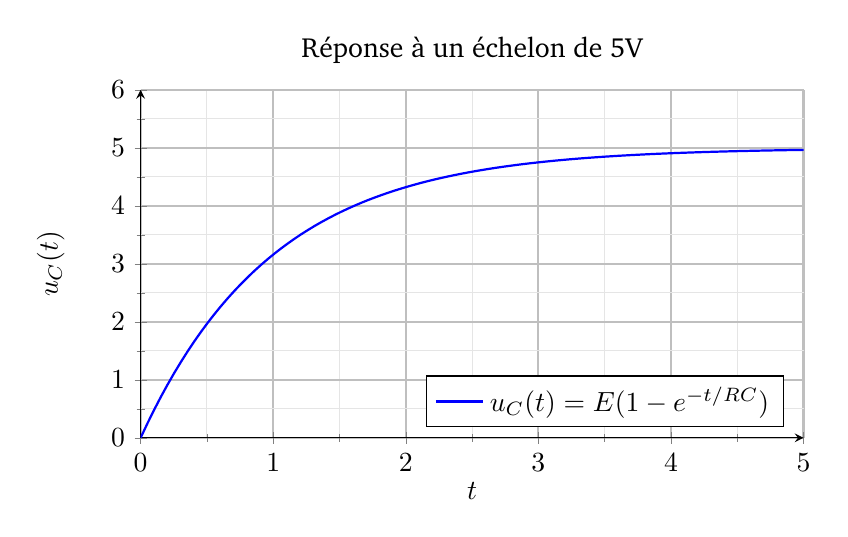
\begin{tikzpicture}
    \begin{axis}[
        domain=0:5, % Domaine de t
        samples=100, % Nombre de points de la courbe
        axis lines=left,
        xlabel={$t$},
        ylabel={$u_C(t)$},
        grid=major,
        width=10cm,
        height=6cm,
        xlabel style={at={(axis description cs:0.5,-0.1)},anchor=north},
        ylabel style={at={(axis description cs:-0.1,.5)},anchor=south},
        title={Réponse à un échelon de 5V},
        legend pos=south east,
        grid=both,
        major grid style={line width=0.8pt,draw=gray!50},
        minor grid style={line width=0.4pt,draw=gray!20},
        minor tick num=1,
        ymin=0, ymax=6,
        xtick distance=1,
        ytick distance=1,
    ]
        \addplot[blue, thick] {5*(1 - exp(-x))};
        \addlegendentry{$u_C(t) = E (1 - e^{-t/RC})$}
    \end{axis}
\end{tikzpicture}
\end{center}

%-----------------------------------------------------------
\section{Vérification mathématique}

On peut vérifier que la fonction obtenue précédemment répond bien à une solution de l'équation différentielle du circuit et que d'autres ne peuvent pas être solution de cette loi d'évolution du circuit.


\subsection{$u_C(t) = A$ (constante)}

On a alors ${\rm d}u_C(t)/{\rm d}t = 0$

Et : $R \cdot C \cdot \frac{{\rm d}u_C(t)}{{\rm d}t} + u_C(t) = A$

Cela ne fonctionne que si $A = E$, c'est à dire si la capacité est déjà chargée.

\subsection{$u_C(t) = B \cdot t + A$ (loi affine)}

On a alors ${\rm d}u_C(t)/{\rm d}t = B$

Et : $R \cdot C \cdot \frac{{\rm d}u_C(t)}{{\rm d}t} + u_C(t) = A + R \cdot C \cdot B$

Cette relation donne une valeur différente de $E$.

\subsection{$u_C(t) = E \cdot (1 - \exp{\frac{-t}{R \cdot C}}$ (exponentielle)}

On a alors ${\rm d}u_C(t)/{\rm d}t = -E/(R \cdot C) \cdot \exp{\frac{-t}{R \cdot C}}$

Et : $R \cdot C \cdot \frac{{\rm d}u_C(t)}{{\rm d}t} + u_C(t) = E \cdot (1 - \exp{\frac{-t}{R \cdot C}} - E/(R \cdot C) \cdot \exp{\frac{-t}{R \cdot C}}$

On obtient alors : $R \cdot C \cdot \frac{{\rm d}u_C(t)}{{\rm d}t} + u_C(t) = E$

\newpage
%-----------------------------------------------------------
\section{Mesure de la constante de temps}

Afin de pouvoir effectuer une \textbf{mesure fiable}, il est important d'avoir un \textbf{protocole expérimental répétable}.

Dans le cas d'un régime transitoire, on cherche à mesurer de manière précise le temps caractéristique d'établissement d'un état stable vers un autre. On souhaite par la suite pouvoir comparer différents systèmes (par exemple ici, différents couples R-C).

\medskip



\begin{center}
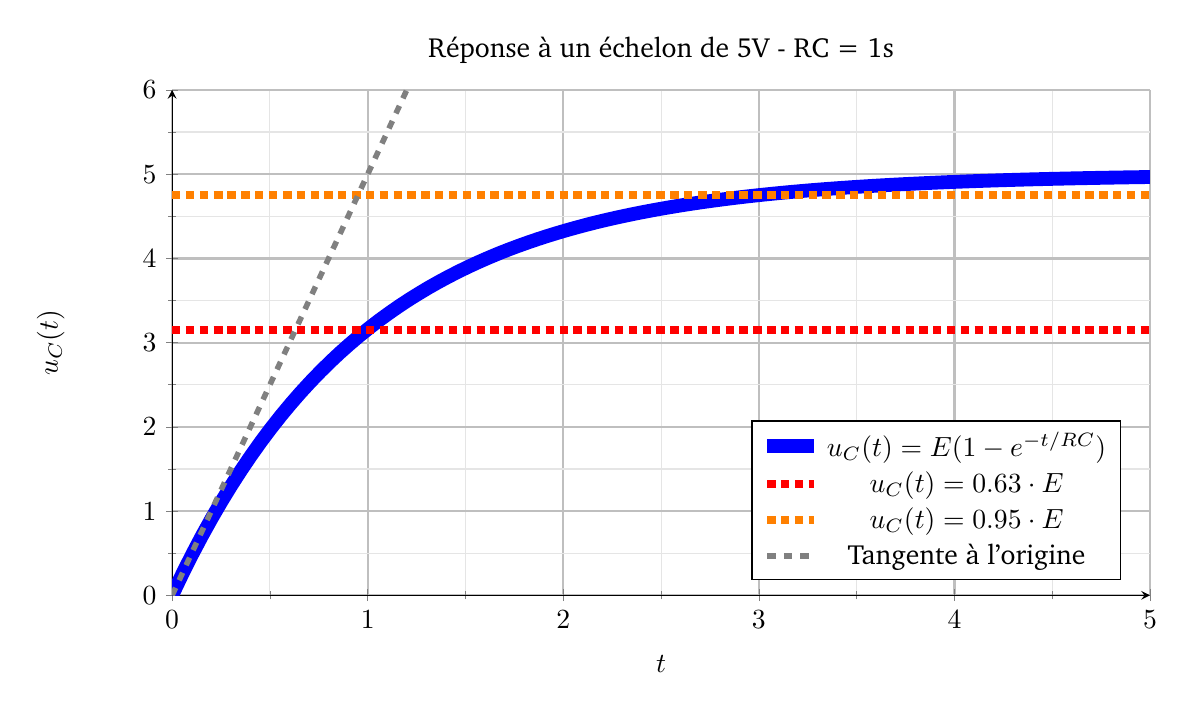
\begin{tikzpicture}
    \begin{axis}[
        domain=0:5, % Domaine de t
        samples=100, % Nombre de points de la courbe
        axis lines=left,
        xlabel={$t$},
        ylabel={$u_C(t)$},
        grid=major,
        width=14cm,
        height=8cm,
        xlabel style={at={(axis description cs:0.5,-0.1)},anchor=north},
        ylabel style={at={(axis description cs:-0.1,.5)},anchor=south},
        title={Réponse à un échelon de 5V - RC = 1s},
        legend pos=south east,
        grid=both,
        major grid style={line width=0.8pt,draw=gray!50},
        minor grid style={line width=0.4pt,draw=gray!20},
        minor tick num=1,
        ymin=0, ymax=6,
        xtick distance=1,
        ytick distance=1,
    ]
        \addplot[blue, line width=5pt] {5*(1 - exp(-x))};
        \addlegendentry{$u_C(t) = E (1 - e^{-t/RC})$}
        
        \addplot[red, line width=3pt, dotted, domain=0:5] {0.63*5};
        \addlegendentry{$u_C(t) = 0.63 \cdot E$}
        
        \addplot[orange, line width=3pt, dotted, domain=0:5] {0.95*5};
        \addlegendentry{$u_C(t) = 0.95 \cdot E$}
        
        \addplot[gray, line width=2pt, dashed, domain=0:5] {5*x};
        \addlegendentry{Tangente à l'origine}
    \end{axis}
\end{tikzpicture}
\end{center}


%-----------------------------------------------------------
\section{Mise en oeuvre}
\subsection{Cablage du montage}

CABLAGE AVEC VOIE DE L'OSCILLOSCOPE 

\subsection{Premier essai avec un générateur de tension continue}

Sans déclenchement (trigger), l'acquisition de la courbe expérimentale est difficile.

\subsection{Déclenchement de l'oscilloscope}

PRENDRE IMAGE OSCILLO + MENU DECLENCHEMENT

\begin{itemize}
	\item Voie de déclenchement
	\item Signal à détecter (souvent front)
	\item Sens de déclenchement (dans le cas d'un front)
	\item Seuil de déclenchement
\end{itemize}

\subsection{Utilisation d'un générateur de fonctions}

NOUVEAU SCHEMA

PRENDRE IMAGE GBF + MENU REGLAGES

PRENDRE IMAGE OSCILLOSCOPE SIGNAL ENTREE/SORTIE

\subsection{Réglage de l'oscilloscope}

PRENDRE IMAGE MENU VOIE

%-----------------------------------------------------------
\section{Compte-rendu}
\subsection{Qu’est-ce qu’un compte rendu ?}
Un compte-rendu est une \textbf{synthèse d'un travail expérimental} que vous avez réalisé. Il permet de résumer les différentes étapes que vous avez été amené à suivre lors des expériences que vous avez menées.


\subsection{A qui s’adresse un compte-rendu ?}
Il s'adresse :

\begin{itemize}
	\item \textbf{à soi-même} : pour pouvoir mener à nouveau l'expérience (avec les mêmes paramètres ou des paramètres différents pour améliorer le modèle physique et mathématique)
	\item \textbf{à une personne extérieure} : pour que cette personne puisse reproduire l'expérience dans des conditions similaires, retrouver les résultats et aboutir aux mêmes analyses
\end{itemize}


\subsection{Quels sont les éléments à inclure dans un compte-rendu ?}\subsubsection{Introduction}

Un compte-rendu doit commencer par une introduction permettant de présenter la problématique abordée ou/et le phénomène physique que l'on souhaite mettre en évidence à travers l'expérience. Cette introduction doit également présenter succinctement la démarche et les résultats que vous cherchez à obtenir.

\subsubsection{Théorie / Modèle mathématique ou/et physique}
Afin d'expliquer la démarche expérimentale et de pouvoir comparer les résultats expérimentaux aux modèles mathématiques et physiques, il faut proposer au lecteur quelques éléments de théorie. Ces éléments doivent se baser sur des outils mathématiques ou/et sur des lois physiques déjà établies.

Cette partie peut aussi être associée à la partie analyse, selon les cas.

\subsubsection{Matériel et méthodes}
Afin de pouvoir répliquer les expériences que vous présentez et les résultats que vous avez obtenus, il est indispensable de présenter l'ensemble du matériel que vous avez utilisé au cours de votre expérience, en incluant la référence des instruments ainsi que leurs paramètres de configuration et les différents consommables que vous avez pu utiliser.

Il faut également présenter les méthodes que vous avez suivies lors de votre expérience, en précisant systématiquement le protocole de mesure utilisé pour chacune des mesures réalisées.

Les outils numériques utilisés doivent aussi être présents dans cette section, que ce soit pour le traitement des données ou la présentation des résultats. Vous pouvez présenter les algorithmes de
traitement de l'information que vous avez utilisé. Les différents codes doivent cependant se trouver en annexe. Seules quelques lignes particulières doivent se retrouver dans cette section.

\subsubsection{Résultats}

Cette section doit présenter les résultats de manière synthétique et clair. Vous devez également décrire les observations sur lesquelles le lecteur doit se focaliser. Il faut l'emmener à voir ce que vous avez vous-même observé.

\subsubsection{Analyse}

Cette section permet de faire le lien entre vos observations expérimentales (ou de simulation) et le modèle théorique sur lequel se base votre expérience (voir section Théorie et Modèles). Il faut synthétiser vos résultats et montrer que votre expérience confirme (ou non) le modèle que vous avez établi.

\subsubsection{Conclusion}

Votre compte-rendu, tout comme votre expérience, doit permettre de répondre à une problématique que vous deviez traiter. Votre compte-rendu doit comporter une conclusion permettant d'établir si la problématique initiale trouve une réponse suite à votre expérience.

\end{document} 